\subsection{Algorithmic Optimizations} \label{subsec:algopti}
According to \textcite{shawahna_fpga-based_2019}, 90\% of computation time in \acrshort{cnn} is consumed by the convolution operation. Therefore, decreasing the number of operations in a convolution will reduce the computational complexity of \acrshort{cnn}. This section investigates algorithms that accelerate the convolution operation.
%
%
\subsubsection{GEMM}
%
\acrfull{gemm} is commonly used to to process \acrshort{cnn} on \acrshort{cpu} and \acrshort{gpu} \cite{abdelouahab_accelerating_2018}. The \acrshort{gemm} converts the convolution operation as a matrix-vector multiplication. In other words, a mini-batch of input \acrshort{fm} and kernels are transformed into two 2D matrices, as illustrated in Figure \ref{fig:gemm}. It is done in such a way that the multiplication between those two matrices gives the same result as a standard convolution. 
%
\begin{figure}[H]
    \centering
    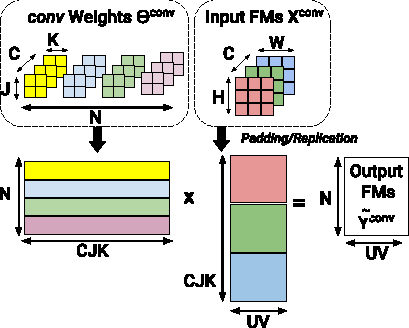
\includegraphics[width=0.5\textwidth]{gemm.pdf}
    \caption{\acrshort{gemm}-based processing of a standard convolution layer, from \cite{abdelouahab_accelerating_2018}}
    \label{fig:gemm}
\end{figure}
%
The advantage of this method becomes more significant as the size of the mini-batch grows \cite{abdelouahab_accelerating_2018}. However, this approach is not appropriate for \acrshort{fpga}. Indeed, \textcite{zhu_efficient_2020, sze_efficient_2017} pointed out that the \acrshort{fm}s, when converted to a vector, must be copied multiple times. It leads to huge memory storage requirements, memory footprint, and complex memory management access patterns. Furthermore, it does not reduce the arithmetic complexity of the convolution \cite{liang_evaluating_2020}.
%
\subsubsection{Fast algorithms for convolution}
%
%
As mentioned previously, the \acrshort{gemm} can accelerate the convolution but it does not reduce the number of operations. Therefore, we can investigate algorithms that aim at computing the convolution operation with fewer operations, named \textbf{fast convolution algorithms}. According to \textcite{liang_evaluating_2020}, there exist two fast convolution algorithms that perform efficiently the 2D convolution: Winograd minimal filter algorithm and \acrfull{fft}. 

The idea behind of these fast convolution algorithms is to transform a kernel and a tile of input into a target domain, where the convolution correponds to an element-wise multiplication in that domain \cite{abdelouahab_accelerating_2018}. At the end, we can obtain the corresponding tile of output by applying the inverse transformation on the product tile. As a result, the fast algorithm produces a tile of output (rather than a single pixel) and reduces the total number of operations by computing an element-wise multiplication (rather than a multiplication followed by an addition).

Therefore, both fast convolutions can be described by a common formula, as expressed in Equation \eqref{eq:comform}, where $T_o$ (resp. $T_I$) is the output (resp. the input) tile, $K$ is the kernel, $\mathcal{H}$ (resp. $\mathcal{H}^{-1}$) is the domain transformation (resp. the inverse transformation) required to perform the algorithms, and $\odot$ is the element-wise multiplication \cite{liang_evaluating_2020}.
%
\begin{equation}
    T_O = \mathcal{H}^{-1} [ \ \mathcal{H}(T_I) \ \odot \ \mathcal{H}(K) \ ]
    \label{eq:comform}
\end{equation}
%
\subsubsection{Winograd-based convolution}
%
The Winograd minimal filter algorithm was first introduced by \cite{winograd_arithmetic_1980}. According to Equation \eqref{eq:comform} and \textcite{abdelouahab_accelerating_2018}, the algorithmn can be defined using the following steps:
\begin{itemize}
    \item An input \acrshort{fm} tile $g$ of size $(T_{ix} \times T_{iy})$ is pre-processed: $$\mathcal{H}(T_I) = \boldsymbol{G^{T}} T_I \boldsymbol{G} $$
    \item In the same way, the kernel $K$, of size $(K_x \times K_y)$ is also transformed: $$\mathcal{H}(K) = \boldsymbol{B^{T}} K \boldsymbol{B}$$
    \item The inverse transformation function is then applied to obtain the output tile: $$\mathcal{H}^{-1}(E) = \boldsymbol{A^{T}} E \boldsymbol{G}$$ Where $E$ is the result of the element-wise multiplication of the two transformed tiles. $$ E = \mathcal{H}(T_I) \ \odot \ \mathcal{H}(K) $$
\end{itemize}
As a result, the output tile $T_O$, of the Winograd Filtering algorithm denoted $F(T_{ix} \times T_{iy}, K_x \times K_y)$, is computed using Equation \eqref{eqn:winograd} \cite{winograd_arithmetic_1980}. The advantage of using the Winograd-based convolution is that the transformation matrix $\boldsymbol{G}$, $\boldsymbol{B}$, $\boldsymbol{A}$ can be computed off-line once $(T_{ix}, T_{iy}, K_x, K_y)$ are fixed, using the Winograd Algorithm \cite{winograd_arithmetic_1980}. Therefore, these domain transform operations become multiplications with a constant and can be optimized on \acrshort{fpga} \cite{liang_evaluating_2020}.
%
\begin{equation}
    T_O = \boldsymbol{A^{T}} [ \ \boldsymbol{G^{T}} T_I \boldsymbol{G} \odot \boldsymbol{B^{T}} K\boldsymbol{B} \ ] \boldsymbol{A}
    \label{eqn:winograd}
\end{equation}

According to \textcite{winograd_arithmetic_1980}, the Winograd convolution reduces the number of multiplications at the cost of an increase in the numbers of additions. The gain obtained is defined in Equation \eqref{eq:winograd_gain} \cite{winograd_arithmetic_1980}. For example, if $T_{ix} = T_{iy} = 2$ and $N_{kx} = N_{ky} = 3$, the complexity reduction factor $F_{multiplication}$ equals $2.25$ \cite{lavin_fast_2016}.
%
\begin{equation}
    F_{multiplication} = \frac{T_{ix} \times T_{iy} \times N_{kx} \times N_{ky}}{(T_{ix} + N_{kx} - 1) \times (T_{iy} + N_{ky} - 1)}
    \label{eq:winograd_gain}
\end{equation}
%
\subsubsection{FFT-based convolution}
%
The \acrshort{fft}, introduced by \textcite{cooley_algorithm_1965}, is an algorithm used to compute the discrete Fourier transform. As presented earlier, once the tile and kernel are in the frequency-domain, the operation corresponding to the convolution is the element-wise multiplication. Therefore, we can use the \acrshort{fft} to perform the convolution operation described in Equation \eqref{eq:comform}, where \cite{liang_evaluating_2020}:
\begin{itemize}
    \item $\mathcal{H}(*) = FFT(*)$
    \item $\mathcal{H}^{-1}(*) = IFFT(*)$
\end{itemize}
%
Using \acrshort{fft}, the computational complexity factor can be reduced from $O(N_{ix} \times N_{iy} \times N_{kx} \times N_{ky})$ to $O(N_{i\{x,y\}} log_2(N_{k\{x,y\}}))$ \cite{w_smith_scientist_1997}.
%
\subsubsection{Comparison between the two fast convolution algorithms}
%
Winograd-based convolution seems to be a preferred way to perform fast convolution. Indeed, \textcite{lavin_fast_2016} demonstrated that Winograd convolution is more efficient when the kernel and the stride are small ($K_* \leq 3$ for the kernel) while \acrshort{fft}-based convolution is more adequate when the kernel is large \cite{ahmad_towards_2019, chitsaz_acceleration_2020}. However, current \acrshort{cnn} trends use small kernels \cite{sandler_mobilenetv2_2018, liang_evaluating_2020} and so, the Winograd convolution.

Moreover, there are examples of successful \acrshort{fpga} implementations of Winograd algorithm: \textcite{liang_evaluating_2020, aydonat_opencl_2017} used Winograd transform and reduced their computational complexity by around 50\%. However, the Winograd algorithm also increased bandwidth utilization \cite{xiao_exploring_2017}.

Yet, \textcite{liang_evaluating_2020, chitsaz_acceleration_2020, zeng_optimizing_2017} worked on the optimization of the frequency-domain convolution on \acrshort{fpga} with small filter by using \acrfull{oad} technique \cite{w_smith_scientist_1997} to lower the number of operations and increase the data parallelism. However, according to \textcite{liang_evaluating_2020, podili_fast_2017}, \acrshort{fft}-based convolution still requires more memory, bandwidth, and logic resources (additions and multiplications) than Winograd. Furthermore, \textcite{zhang_caffeine_2016} pointed out that performing \acrshort{fft} convolution with $1 \times 1$ kernel is inefficient, and they performed it in time-domain only.
